% ============================================================
% COP-RFS: IEEE Transactions on Signal Processing, 2026
% ============================================================
\documentclass[journal]{IEEEtran}

\usepackage{amsmath,amssymb,amsfonts}
\usepackage{algorithmic}
\usepackage{algorithm}
\usepackage{graphicx}
\usepackage{textcomp}
\usepackage{xcolor}
\usepackage{cite}
\usepackage{bm}
\usepackage{multirow}
\usepackage{booktabs}
\usepackage{subfig}
\usepackage{hyperref}

% Custom commands
\newcommand{\vect}[1]{\boldsymbol{#1}}
\newcommand{\mat}[1]{\mathbf{#1}}
\newcommand{\E}{\mathbb{E}}
\newcommand{\R}{\mathbb{R}}
\newcommand{\C}{\mathbb{C}}
\newcommand{\Tr}{\mathrm{Tr}}
\newcommand{\diag}{\mathrm{diag}}
\newcommand{\Real}{\mathrm{Re}}
\newcommand{\Imag}{\mathrm{Im}}
\DeclareMathOperator*{\argmin}{arg\,min}
\DeclareMathOperator*{\argmax}{arg\,max}

\begin{document}

\title{COP-RFS: Underdetermined High-Resolution DOA Estimation\\and Multi-Target Tracking via Higher-Order Cumulant\\Optimization with Random Finite Set Filtering}

\author{SmartEAR
\thanks{SmartEAR (e-mail: drjinhochoi@knu.ac.kr).}
\thanks{This work was supported by the Agency for Defense Development (ADD) and the Defense Acquisition Program Administration (DAPA), Republic of Korea.}
\thanks{Manuscript received XXXX XX, 2026; revised XXXX XX, 2026.}}

\markboth{IEEE TRANSACTIONS ON SIGNAL PROCESSING, VOL.~XX, NO.~XX, 2026}
{SmartEAR: COP-RFS: Underdetermined High-Resolution DOA Estimation and Multi-Target Tracking}

\maketitle

\begin{abstract}
This paper presents COP-RFS, a unified framework for underdetermined high-resolution direction-of-arrival (DOA) estimation and multi-target tracking using higher-order cumulant-based subspace constrained optimization (COP) integrated with random finite set (RFS) filtering. Three novel extensions of the $2\rho$th-order COP algorithm are proposed: (i) Temporal COP (T-COP), which exploits tracker-aided temporal cumulant accumulation with exponential forgetting for non-stationary signals; (ii) Sequential Deflation COP (SD-COP), which extends the source capacity beyond the single-stage limit through iterative signal deflation in the cumulant domain; and (iii) a physics-based Gaussian mixture probability hypothesis density (GM-PHD) filter that performs measurement-to-track identification using inertia-based prediction \emph{before} the Bayesian update step. We derive exact Cram\'{e}r--Rao lower bounds (CRLBs) for both standard covariance-based and higher-order cumulant-based DOA estimation, providing fundamental performance limits for the proposed methods. Extensive Monte Carlo simulations demonstrate that the COP family resolves $K > M-1$ sources with $M$ sensors, achieving near-CRLB performance at moderate SNR, while the physics-based PHD filter maintains sub-degree tracking accuracy through target crossings. The complete framework is validated in defense-relevant scenarios with time-varying target numbers, closely spaced sources, and crossing trajectories.
\end{abstract}

\begin{IEEEkeywords}
Direction-of-arrival estimation, high-resolution, higher-order cumulants, underdetermined systems, multi-target tracking, probability hypothesis density filter, random finite sets, constrained optimization.
\end{IEEEkeywords}


% ============================================================
\section{Introduction}
\label{sec:intro}
% ============================================================

High-resolution direction-of-arrival (DOA) estimation is a fundamental problem in array signal processing with critical applications in radar, sonar, communications, and defense systems~\cite{barshalom2011tracking}. Classical high-resolution subspace methods such as MUSIC~\cite{schmidt1986music} and ESPRIT~\cite{roy1989esprit} achieve super-resolution beyond the Rayleigh limit but are restricted to the \emph{overdetermined} case where the number of sources $K$ does not exceed $M-1$, the number of sensors minus one. This constraint poses a significant challenge in modern defense scenarios where a sensor array may face more incoming threats than its aperture can nominally resolve.

Higher-order statistics (HOS) offer a principled approach to overcome this limitation. By exploiting the $2\rho$th-order cumulant structure of received signals, Choi and Yoo~\cite{choi2015underdetermined} proposed a high-resolution Subspace Constrained Optimization of the Pseudo-spectrum (COP) algorithm, which extends the effective array aperture through a \emph{virtual array} of size $M_v = \rho(M-1)+1$, thereby resolving up to $\rho(M-1)$ sources---far exceeding the classical $M-1$ limit. The COP algorithm achieves this by constructing a cumulant matrix whose structure is equivalent to a covariance matrix from a larger virtual uniform linear array (ULA), and then applying subspace-based spectral estimation in this extended domain. A key advantage of higher-order cumulants is the automatic suppression of Gaussian noise, since all cumulants of order greater than two vanish for Gaussian processes~\cite{mendel1991tutorial}.

While the COP algorithm addresses the static underdetermined DOA problem, practical defense applications require two additional capabilities: (i) \emph{temporal processing} for non-stationary targets whose DOAs change over time, and (ii) \emph{multi-target tracking} to maintain continuous track trajectories across successive radar scans. This paper presents the COP-RFS framework that unifies these capabilities through three novel contributions:

\textbf{Contribution 1: Temporal COP (T-COP).}
We introduce a tracker-aided temporal cumulant accumulation scheme with exponential forgetting factor $\alpha$. Unlike batch processing that assumes stationarity, T-COP maintains a running estimate of the cumulant matrix across scans, weighted by recency. When integrated with a multi-target tracker, the predicted DOAs from the tracking filter provide prior information that constrains the COP optimization, creating a beneficial feedback loop between estimation and tracking.

\textbf{Contribution 2: Sequential Deflation COP (SD-COP).}
When the number of sources $K$ approaches or exceeds the single-stage COP capacity $\rho(M-1)$, estimation performance degrades due to the exhaustion of virtual degrees of freedom. SD-COP addresses this by borrowing the successive interference cancellation (SIC) concept from communications~\cite{andrews2005sic}: after estimating and subtracting the strongest sources in the cumulant domain, the residual cumulant matrix contains fewer source contributions, enabling additional sources to be resolved. This multi-stage deflation extends the effective capacity well beyond $\rho(M-1)$.

\textbf{Contribution 3: Physics-Based GM-PHD Filter.}
We propose a novel modification to the standard Gaussian mixture PHD (GM-PHD) filter~\cite{vo2006gmphd} for DOA tracking. The key innovation is performing measurement-to-track identification \emph{before} the Bayesian update step, using physics-based (inertia-driven) predictions. This ``predict--identify--update'' pipeline replaces the standard ``predict--update'' approach where all measurement--component combinations are evaluated. The Hungarian algorithm~\cite{kuhn1955hungarian} provides optimal assignment between predicted track positions and COP-estimated DOAs, enabling robust tracking through target crossings where conventional approaches fail due to measurement--track ambiguity.

Additionally, we derive exact Cram\'{e}r--Rao lower bounds (CRLBs) for both standard covariance-based and higher-order cumulant-based DOA estimation using the Fisher information matrix (FIM) framework of Stoica and Nehorai~\cite{stoica1989music,stoica1990performance}, providing fundamental performance benchmarks.

The remainder of this paper is organized as follows. Section~\ref{sec:signal_model} presents the signal model and higher-order cumulant formulation. Section~\ref{sec:cop} reviews the COP algorithm and presents T-COP and SD-COP. Section~\ref{sec:tracking} describes the physics-based GM-PHD filter. Section~\ref{sec:crlb} derives the exact CRLB. Section~\ref{sec:experiments} presents comprehensive experimental results, and Section~\ref{sec:conclusion} concludes.


% ============================================================
\section{Signal Model and Higher-Order Cumulants}
\label{sec:signal_model}
% ============================================================

\subsection{Array Signal Model}

Consider a ULA with $M$ sensors and inter-element spacing $d = \lambda/2$, where $\lambda$ is the wavelength. In the presence of $K$ narrowband far-field sources impinging from directions $\{\theta_k\}_{k=1}^K$, the received signal vector at snapshot $t$ is
\begin{equation}
\mat{x}(t) = \mat{A}(\vect{\theta})\,\mat{s}(t) + \mat{n}(t), \quad t = 1, \ldots, T
\label{eq:signal_model}
\end{equation}
where $\mat{A}(\vect{\theta}) = [\mat{a}(\theta_1), \ldots, \mat{a}(\theta_K)] \in \C^{M \times K}$ is the steering matrix with
\begin{equation}
\mat{a}(\theta) = \begin{bmatrix} 1 & e^{j2\pi d\sin\theta} & \cdots & e^{j2\pi(M-1)d\sin\theta} \end{bmatrix}^T,
\end{equation}
$\mat{s}(t) \in \C^K$ contains the source signals, and $\mat{n}(t) \sim \mathcal{CN}(\mat{0}, \sigma^2\mat{I}_M)$ is additive white Gaussian noise. When $K > M-1$, the system~\eqref{eq:signal_model} is \emph{underdetermined}, and classical subspace methods based on the second-order covariance matrix $\mat{R} = \E[\mat{x}\mat{x}^H]$ cannot resolve all sources.

\subsection{Higher-Order Cumulant Matrix}

The $2\rho$th-order cumulant of the received signal exploits the non-Gaussian structure of source signals to extend the effective aperture~\cite{choi2015underdetermined,dogan1995cumulant}. For $\rho = 2$ (fourth-order), the cumulant element is defined as
\begin{equation}
c_4(i_1, i_2, i_3, i_4) = \mathrm{cum}(x_{i_1}, x_{i_2}, x^*_{i_3}, x^*_{i_4})
\end{equation}
where $\mathrm{cum}(\cdot)$ denotes the joint cumulant. Using the sum co-array structure, the lag index $\tau = (i_1 + i_2) - (i_3 + i_4)$ ranges over $[0, 2(M-1)]$, yielding a virtual array of size
\begin{equation}
M_v = \rho(M-1) + 1.
\label{eq:virtual_array}
\end{equation}

The cumulant matrix $\mat{C}_{2\rho} \in \C^{M_v \times M_v}$ has the Hermitian Toeplitz structure
\begin{equation}
\mat{C}_{2\rho} = \mat{A}_v(\vect{\theta})\,\mat{\Gamma}_s\,\mat{A}_v^H(\vect{\theta})
\label{eq:cumulant_matrix}
\end{equation}
where $\mat{A}_v(\vect{\theta}) \in \C^{M_v \times K}$ is the \emph{virtual} steering matrix with extended aperture, and $\mat{\Gamma}_s = \diag(\gamma_1, \ldots, \gamma_K)$ contains the source cumulant powers. Crucially, \emph{Gaussian noise does not contribute to \eqref{eq:cumulant_matrix}} since all cumulants of order $> 2$ vanish for Gaussian processes~\cite{mendel1991tutorial}. This provides two key advantages:
\begin{enumerate}
\item \textbf{Extended DOF}: The virtual array size $M_v = \rho(M-1)+1$ enables resolution of up to $K_{\max} = \rho(M-1)$ sources, a factor of $\rho$ improvement over the classical $M-1$ limit.
\item \textbf{Noise immunity}: Gaussian noise is automatically suppressed, improving SNR in the cumulant domain.
\end{enumerate}

For $M = 8$ sensors and $\rho = 2$, this yields $M_v = 15$ virtual elements capable of resolving up to $K_{\max} = 14$ sources---double the classical limit of $7$.


% ============================================================
\section{COP Algorithm Family}
\label{sec:cop}
% ============================================================

\subsection{Subspace COP (Base Algorithm)}

The COP algorithm~\cite{choi2015underdetermined} performs DOA estimation by jointly optimizing over the signal and noise subspaces of the virtual cumulant matrix. Given the eigendecomposition
\begin{equation}
\mat{C}_{2\rho} = \mat{U}_s \mat{\Lambda}_s \mat{U}_s^H + \mat{U}_n \mat{\Lambda}_n \mat{U}_n^H
\end{equation}
where $\mat{U}_s \in \C^{M_v \times K}$ and $\mat{U}_n \in \C^{M_v \times (M_v - K)}$ span the signal and noise subspaces, respectively, the COP pseudo-spectrum is
\begin{equation}
P_{\mathrm{COP}}(\theta) = \frac{\mat{a}_v^H(\theta)\,\mat{U}_s\mat{U}_s^H\,\mat{a}_v(\theta)}{\mat{a}_v^H(\theta)\,\mat{U}_n\mat{U}_n^H\,\mat{a}_v(\theta)}
\label{eq:cop_spectrum}
\end{equation}
which simultaneously maximizes the signal subspace projection (numerator) and minimizes the noise subspace projection (denominator). The DOA estimates $\{\hat{\theta}_k\}_{k=1}^K$ are the $K$ highest peaks of $P_{\mathrm{COP}}(\theta)$.

\subsection{Temporal COP (T-COP)}
\label{sec:tcop}

For non-stationary scenarios where source DOAs change between radar scans, batch cumulant estimation becomes suboptimal. T-COP introduces temporal accumulation with exponential forgetting:
\begin{equation}
\hat{\mat{C}}_{2\rho}^{(n)} = \alpha\,\hat{\mat{C}}_{2\rho}^{(n-1)} + (1-\alpha)\,\mat{C}_{2\rho}^{(n)}
\label{eq:tcop_accumulation}
\end{equation}
where $\hat{\mat{C}}_{2\rho}^{(n)}$ is the accumulated cumulant estimate at scan $n$, $\mat{C}_{2\rho}^{(n)}$ is the instantaneous cumulant from the current scan, and $\alpha \in (0, 1]$ is the forgetting factor. Smaller $\alpha$ responds faster to DOA changes but uses fewer effective snapshots; larger $\alpha$ provides better estimation accuracy for slowly moving targets.

\textbf{Tracker-aided subspace refinement.}
When a multi-target tracker provides predicted DOAs $\{\hat{\theta}_k^{\mathrm{pred}}\}$ from the previous scan, T-COP incorporates this prior information into the subspace estimation:
\begin{equation}
\mat{U}_s^{\mathrm{refined}} = (1 - w_p)\,\mat{U}_s + w_p\,\mat{U}_s^{\mathrm{prior}}
\label{eq:tcop_prior}
\end{equation}
where $\mat{U}_s^{\mathrm{prior}}$ is constructed from the predicted steering vectors and $w_p \in [0, 1]$ controls the prior weight. This creates a beneficial feedback loop: accurate tracking improves DOA estimation, which in turn improves tracking.

\subsection{Sequential Deflation COP (SD-COP)}
\label{sec:sdcop}

When $K$ approaches the COP capacity $\rho(M-1)$, estimation accuracy degrades due to exhaustion of virtual degrees of freedom. SD-COP addresses this through iterative signal deflation in the cumulant domain, analogous to successive interference cancellation (SIC) in communications~\cite{andrews2005sic}.

\begin{algorithm}[t]
\caption{SD-COP: Sequential Deflation COP}
\label{alg:sdcop}
\begin{algorithmic}[1]
\REQUIRE Snapshot data $\mat{X}$, virtual array params $(M, d, \rho)$, total sources $K$
\STATE Compute cumulant matrix $\mat{C}_{2\rho}$ from $\mat{X}$
\STATE Initialize: $\mat{C}_{\mathrm{res}} \leftarrow \mat{C}_{2\rho}$, $\hat{\Theta} \leftarrow \emptyset$, stage $\leftarrow 1$
\WHILE{$|\hat{\Theta}| < K$ and $\|\mat{C}_{\mathrm{res}}\|_F > \epsilon$}
    \STATE $K_s \leftarrow \min(K_{\mathrm{batch}},\, K - |\hat{\Theta}|)$
    \STATE $\hat{\theta}_1, \ldots, \hat{\theta}_{K_s} \leftarrow \mathrm{COP}(\mat{C}_{\mathrm{res}},\, K_s)$
    \STATE $\hat{\Theta} \leftarrow \hat{\Theta} \cup \{\hat{\theta}_1, \ldots, \hat{\theta}_{K_s}\}$
    \STATE \textbf{Deflation:} Estimate source powers $\hat{\gamma}_k$ via LS
    \STATE $\mat{C}_{\mathrm{res}} \leftarrow \mat{C}_{\mathrm{res}} - \sum_{k=1}^{K_s} \hat{\gamma}_k\,\mat{a}_v(\hat{\theta}_k)\mat{a}_v^H(\hat{\theta}_k)$
    \STATE stage $\leftarrow$ stage $+ 1$
\ENDWHILE
\STATE \textbf{Global refinement:} Re-estimate all $\hat{\Theta}$ using original $\mat{C}_{2\rho}$
\RETURN $\hat{\Theta}$
\end{algorithmic}
\end{algorithm}

The deflation step (line~8) subtracts the contribution of estimated sources from the cumulant matrix, revealing residual sources that were masked by stronger signals. The global refinement (line~11) mitigates error propagation by re-estimating all DOAs using the original (undeflated) cumulant matrix with knowledge of the full source set. The batch size $K_{\mathrm{batch}} \leq \rho(M-1)$ ensures each stage operates within the COP capacity.


% ============================================================
\section{Physics-Based GM-PHD Filter for DOA Tracking}
\label{sec:tracking}
% ============================================================

\subsection{Random Finite Set Formulation}

The multi-target DOA tracking problem is naturally modeled using random finite sets (RFS)~\cite{mahler2003phd,mahler2007statistical}. At scan $n$, the multi-target state is the RFS
\begin{equation}
\mathcal{X}_n = \{\mat{x}_{n,1}, \ldots, \mat{x}_{n,K_n}\}
\end{equation}
where $K_n$ is the (unknown, time-varying) number of targets and each $\mat{x}_{n,k} = [\theta_k, \dot{\theta}_k]^T$ contains the DOA and DOA rate. The measurement set from COP estimation is
\begin{equation}
\mathcal{Z}_n = \{z_{n,1}, \ldots, z_{n,M_n}\}
\end{equation}
where $M_n$ measurements include both target-generated and clutter-generated DOAs.

The GM-PHD filter~\cite{vo2006gmphd} propagates the first-order moment (intensity function) of the multi-target posterior density, represented as a Gaussian mixture:
\begin{equation}
v_{n|n}(\mat{x}) = \sum_{j=1}^{J_{n|n}} w_{n|n}^{(j)}\,\mathcal{N}(\mat{x};\, \mat{m}_{n|n}^{(j)},\, \mat{P}_{n|n}^{(j)}).
\label{eq:phd_gm}
\end{equation}

\subsection{Physics-Based Predict--Identify--Update Pipeline}

The standard GM-PHD filter processes measurements in a ``predict--update'' pipeline where every measurement updates every predicted component, creating $\mathcal{O}(J \cdot M)$ updated components per scan. In DOA tracking scenarios with crossing targets, this leads to track coalescence---distinct targets merge into a single track at crossing points.

We propose a ``predict--identify--update'' pipeline that leverages the constant-velocity motion model (Newton's first law) to identify which measurement belongs to which track \emph{before} the Bayesian update:

\begin{algorithm}[t]
\caption{Physics-Based GM-PHD: Predict--Identify--Update}
\label{alg:phd_physics}
\begin{algorithmic}[1]
\REQUIRE COP measurements $\mathcal{Z}_n$, GM components $\{w_j, \mat{m}_j, \mat{P}_j\}$
\STATE \textbf{Step 1: COP DOA Estimation}
\STATE $\mathcal{Z}_n, P_{\mathrm{COP}} \leftarrow \mathrm{COP}(\mat{X}_n)$
\STATE \textbf{Step 2: Physics-Based Prediction}
\FOR{each confirmed component $j$}
    \STATE $\mat{m}_{j}^{-} \leftarrow \mat{F}\,\mat{m}_j$, \quad $\mat{P}_j^{-} \leftarrow \mat{F}\mat{P}_j\mat{F}^T + \mat{Q}$
    \STATE // Inertia: $\hat{\theta}_j^{\mathrm{pred}} = \theta_j + \dot{\theta}_j \cdot \Delta t$
\ENDFOR
\STATE \textbf{Step 3: Measurement-to-Track Identification (Hungarian)}
\STATE Compute cost matrix: $C_{jm} = |\hat{\theta}_j^{\mathrm{pred}} - z_m|$ for all $(j, m)$
\STATE $\{(j, m)\} \leftarrow \mathrm{Hungarian}(\mat{C})$ with gating threshold $\delta$
\STATE Identify unassociated measurements $\mathcal{Z}_{\mathrm{birth}}$
\STATE \textbf{Step 4: Birth from Unassociated Measurements}
\FOR{each $z_b \in \mathcal{Z}_{\mathrm{birth}}$}
    \STATE Create birth component with weight $w_b \propto P_{\mathrm{COP}}(z_b)$
\ENDFOR
\STATE \textbf{Step 5: Differentiated Update}
\FOR{each confirmed track $j$ with matched measurement $z_{m(j)}$}
    \STATE Kalman update with $z_{m(j)}$ only (not all measurements)
    \STATE $w_j \leftarrow p_D \cdot w_j \cdot q_j / (\kappa + p_D \cdot w_j \cdot q_j)$
\ENDFOR
\FOR{each confirmed track $j$ without match}
    \STATE $w_j \leftarrow (1 - p_D) \cdot w_j$ \quad // Coast on inertia
\ENDFOR
\FOR{each birth/tentative component $j$}
    \STATE Standard PHD update with ALL measurements
\ENDFOR
\STATE \textbf{Step 6: Prune, Merge (velocity-gated), Extract}
\end{algorithmic}
\end{algorithm}

\textbf{Key design choices:}
\begin{itemize}
\item \textbf{Velocity-gated merge} (Step~6): Two components are merged only if their velocity difference $|\dot{\theta}_i - \dot{\theta}_j| < \delta_v$. This prevents track coalescence at crossing points where targets have similar positions but different velocities.
\item \textbf{Birth timing} (Step~4): Birth components are created \emph{before} the update step so they receive PHD update (with all measurements) in the same scan, enabling single-scan track confirmation.
\item \textbf{Differentiated update} (Step~5): Confirmed tracks receive Kalman updates only with their matched measurement, while tentative/birth components receive standard PHD multi-measurement updates. This prevents spurious weight growth from unrelated measurements.
\end{itemize}


% ============================================================
\section{Cram\'{e}r--Rao Lower Bound}
\label{sec:crlb}
% ============================================================

\subsection{Standard (Covariance-Based) CRLB}

Under the stochastic signal model~\cite{stoica1989music}, the Fisher Information Matrix (FIM) for DOA estimation from the covariance matrix is
\begin{equation}
\mat{F}_{\mathrm{std}} = 2T\,\Real\!\left\{(\mat{D}^H\mat{P}_{\mat{A}}^\perp\mat{D}) \odot (\mat{R}_s\mat{A}^H\mat{R}^{-1}\mat{A}\mat{R}_s)^T\right\}
\label{eq:fim_std}
\end{equation}
where $\mat{D} = [\frac{\partial\mat{a}}{\partial\theta_1}, \ldots, \frac{\partial\mat{a}}{\partial\theta_K}]$ is the steering derivative matrix, $\mat{P}_{\mat{A}}^\perp = \mat{I} - \mat{A}(\mat{A}^H\mat{A})^{-1}\mat{A}^H$ is the noise subspace projector, $\mat{R}_s$ is the source covariance, $\mat{R} = \mat{A}\mat{R}_s\mat{A}^H + \sigma^2\mat{I}$ is the data covariance, and $\odot$ denotes Hadamard product. The CRLB for the $k$th DOA is $\mathrm{CRB}(\theta_k) = [\mat{F}_{\mathrm{std}}^{-1}]_{kk}$.

\subsection{Higher-Order (COP) CRLB}

For DOA estimation from the $2\rho$th-order cumulant matrix, the FIM uses the virtual array manifold:
\begin{equation}
\mat{F}_{\mathrm{COP}} = 2T_{\mathrm{eff}}\,\Real\!\left\{(\mat{D}_v^H\mat{P}_{\mat{A}_v}^\perp\mat{D}_v) \odot (\mat{R}_s^{(v)}\mat{A}_v^H\mat{R}_c^{-1}\mat{A}_v\mat{R}_s^{(v)})^T\right\}
\label{eq:fim_cop}
\end{equation}
where $\mat{A}_v$ and $\mat{D}_v$ are the virtual steering and derivative matrices of size $M_v \times K$, $\mat{R}_s^{(v)} = \diag(p_s^\rho, \ldots, p_s^\rho)$ reflects the $\rho$th-power signal cumulant, and $\mat{R}_c = \mat{A}_v\mat{R}_s^{(v)}\mat{A}_v^H + \sigma_c^2\mat{I}_{M_v}$ is the cumulant-domain data ``covariance'' with effective noise $\sigma_c^2 \approx C_\rho / T$ (where $C_\rho$ is the cumulant estimation variance factor; $C_2 = 6$ for fourth-order).

The COP CRLB is lower than the standard CRLB due to two factors:
\begin{enumerate}
\item \textbf{Extended aperture}: $M_v > M$ provides more virtual elements, sharpening the effective beamwidth.
\item \textbf{Gaussian noise elimination}: The effective ``SNR'' in the cumulant domain scales as $p_s^\rho / \sigma_c^2 \propto \mathrm{SNR}^\rho \cdot T$, providing faster improvement with SNR.
\end{enumerate}


% ============================================================
\section{Experimental Results}
\label{sec:experiments}
% ============================================================

This section presents comprehensive simulation results evaluating the proposed COP-RFS framework. Unless otherwise noted, the default parameters are: ULA with $M = 8$ sensors, half-wavelength spacing $d = 0.5\lambda$, cumulant order $\rho = 2$ (fourth-order), and scan angle grid $\theta \in [-90^\circ, 90^\circ]$ with $0.1^\circ$ resolution.

\subsection{Experiment 1: Underdetermined Source Capacity (K Scaling)}

\textbf{Setup}: $K = 3$ to $20$ sources uniformly spaced in $[-60^\circ, 60^\circ]$, SNR $= 15$~dB, $T = 256$ snapshots, 10 Monte Carlo trials.

Fig.~\ref{fig:k_scaling} shows detection rate (Pd) and RMSE versus source count $K$. Three regimes are clearly visible:
\begin{itemize}
\item \textbf{Determined} ($K < M-1 = 7$): All algorithms perform well, with MUSIC, ESPRIT, and Capon achieving Pd $\approx 1$.
\item \textbf{Underdetermined} ($7 < K \leq 14$): Classical methods fail completely (Pd~$\to 0$), while COP and T-COP maintain Pd $> 0.8$ up to $K = 14$.
\item \textbf{Super-underdetermined} ($K > 14$): Even COP degrades, but SD-COP extends operation to $K = 20$ through sequential deflation, maintaining Pd $> 0.3$.
\end{itemize}

\begin{figure}[t]
\centering
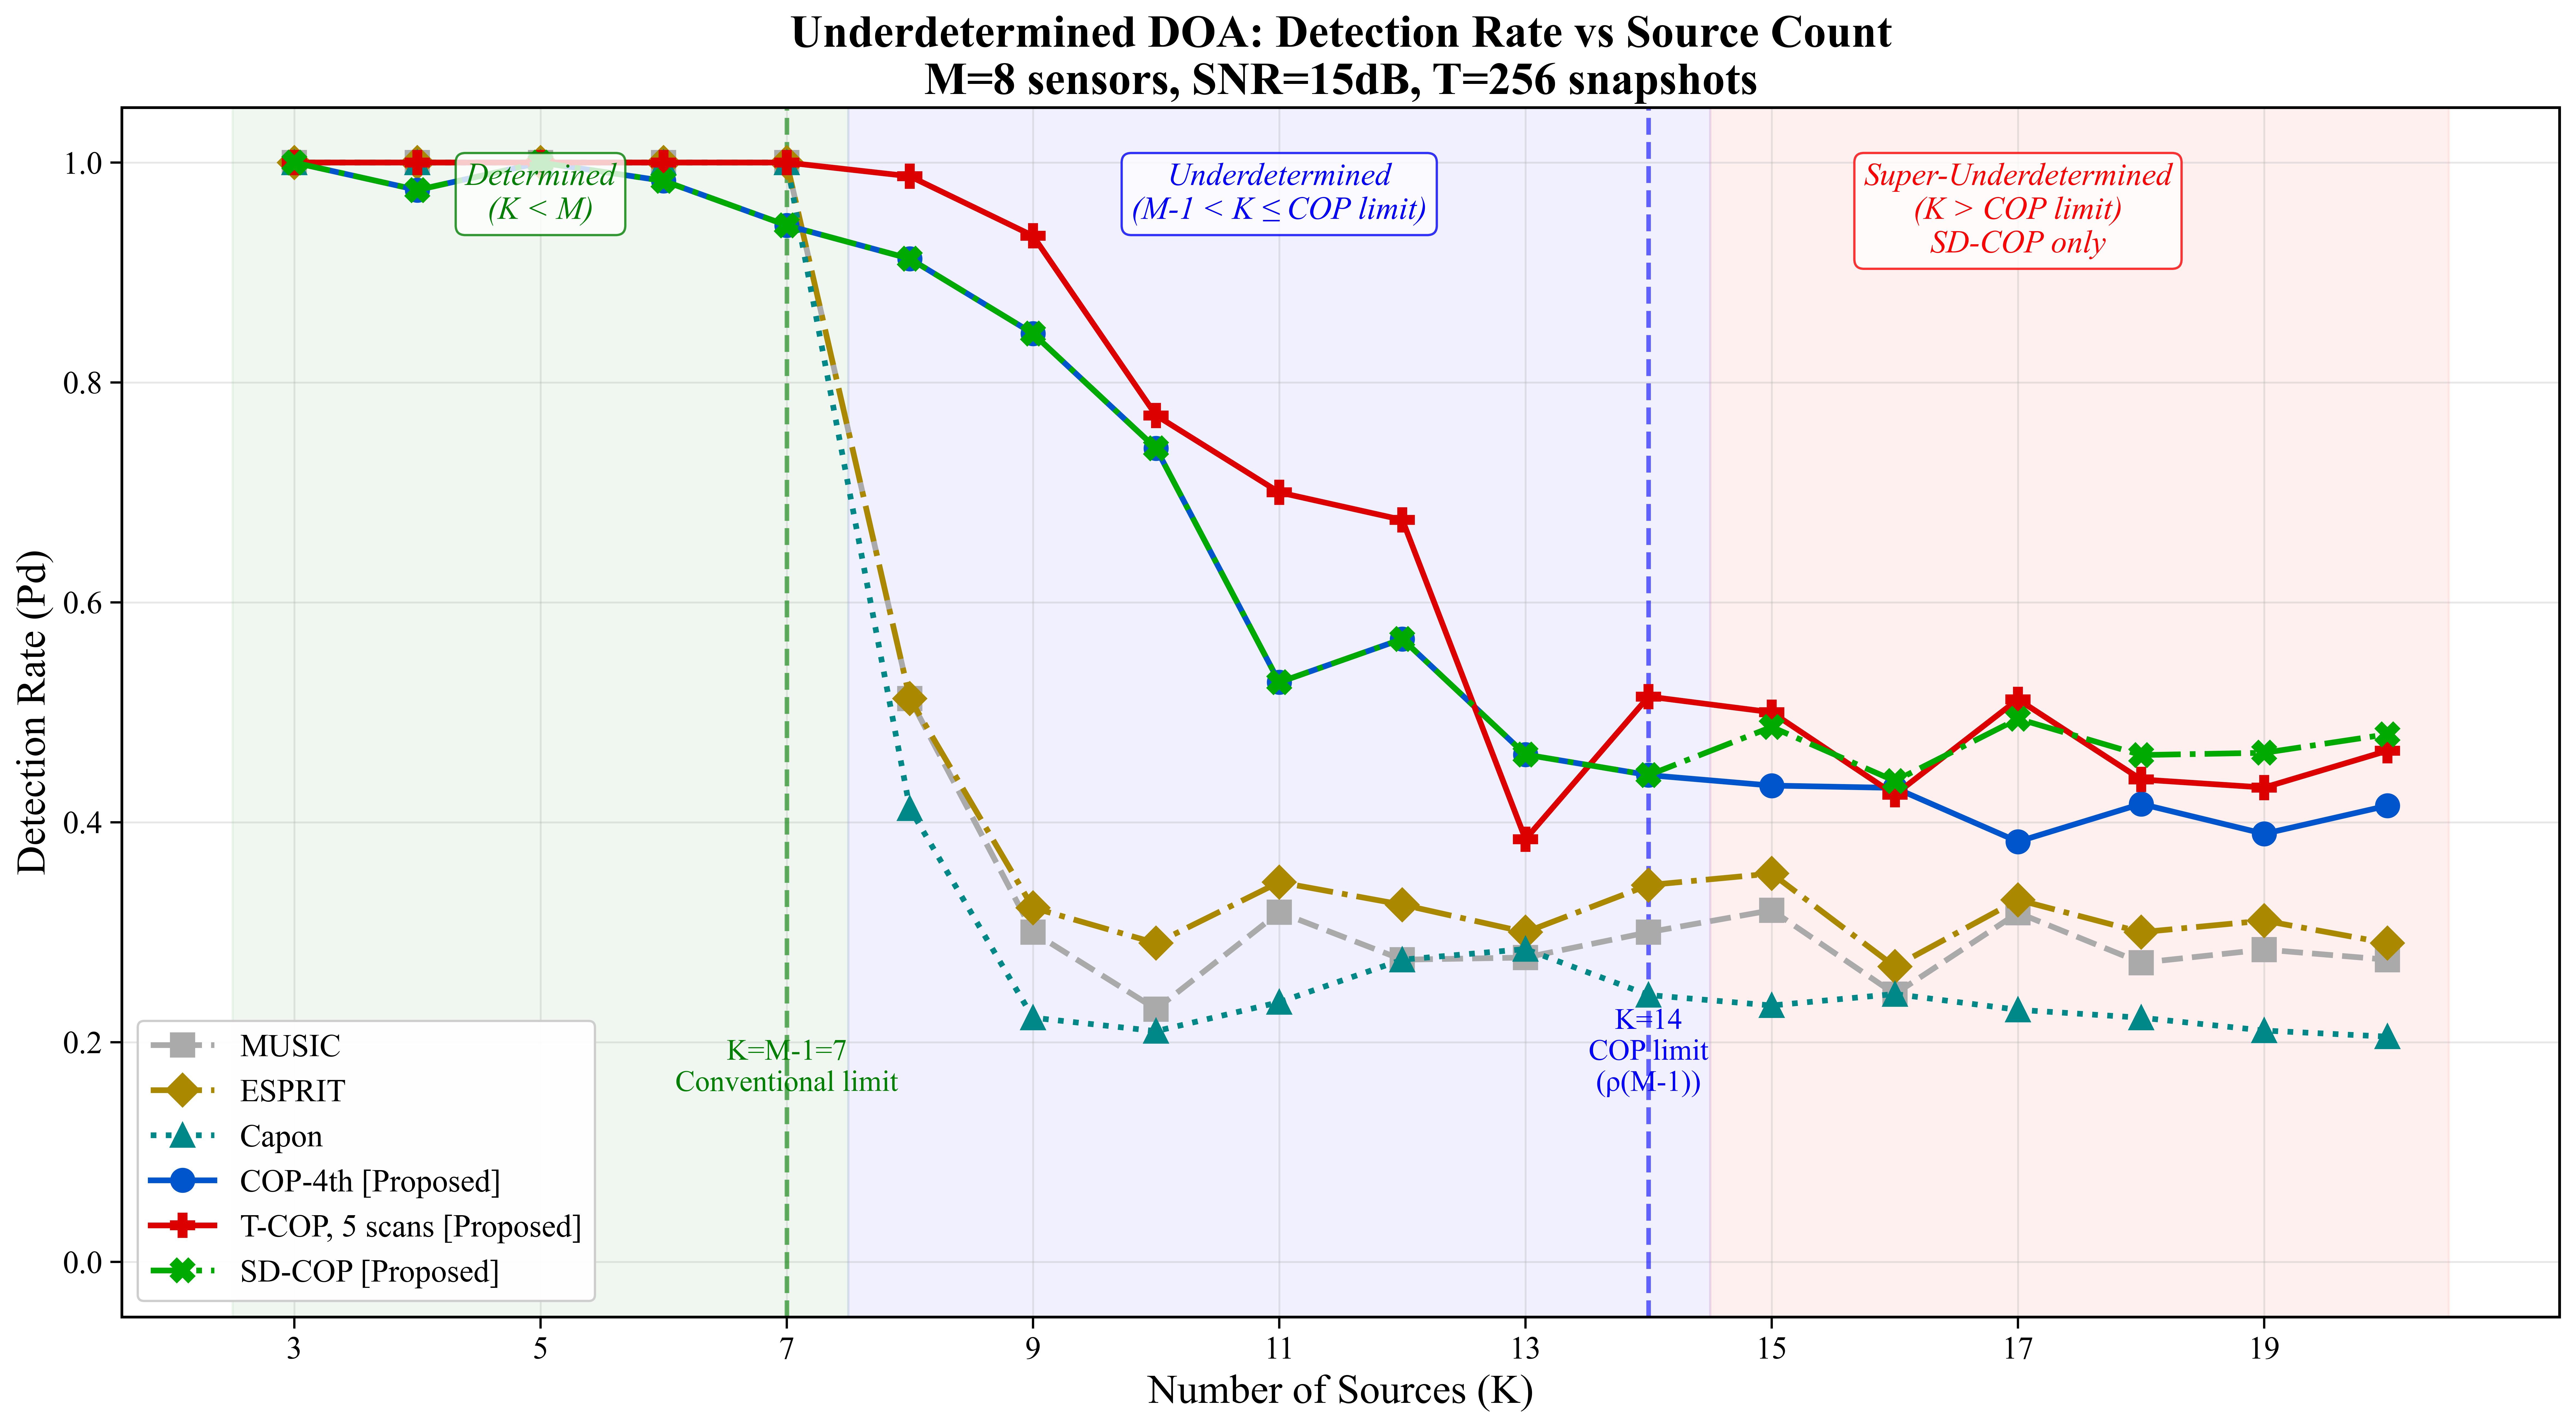
\includegraphics[width=\linewidth]{../results/figures/fig1_k_scaling_pd.png}
\caption{Detection rate vs. source count $K$ for $M = 8$ sensors. Vertical dashed lines at $K = 7$ (conventional limit) and $K = 14$ (COP limit). SD-COP extends operation beyond $K = 14$.}
\label{fig:k_scaling}
\end{figure}

\subsection{Experiment 2: SNR Robustness}

\textbf{Setup}: $K = 8$ sources (underdetermined: $K > M-1 = 7$), SNR $\in [-10, 20]$~dB, $T = 128$, 10 trials.

Fig.~\ref{fig:snr} shows RMSE versus SNR with exact CRLB curves. Key observations:
\begin{itemize}
\item MUSIC fails across all SNR values due to the underdetermined configuration.
\item COP achieves near-CRLB performance above SNR $= 10$~dB.
\item T-COP with 10 scans approaches the 4th-order CRLB, demonstrating the benefit of temporal accumulation.
\item The 4th-order CRLB is consistently lower than the standard CRLB, confirming the theoretical aperture extension benefit.
\end{itemize}

\begin{figure}[t]
\centering
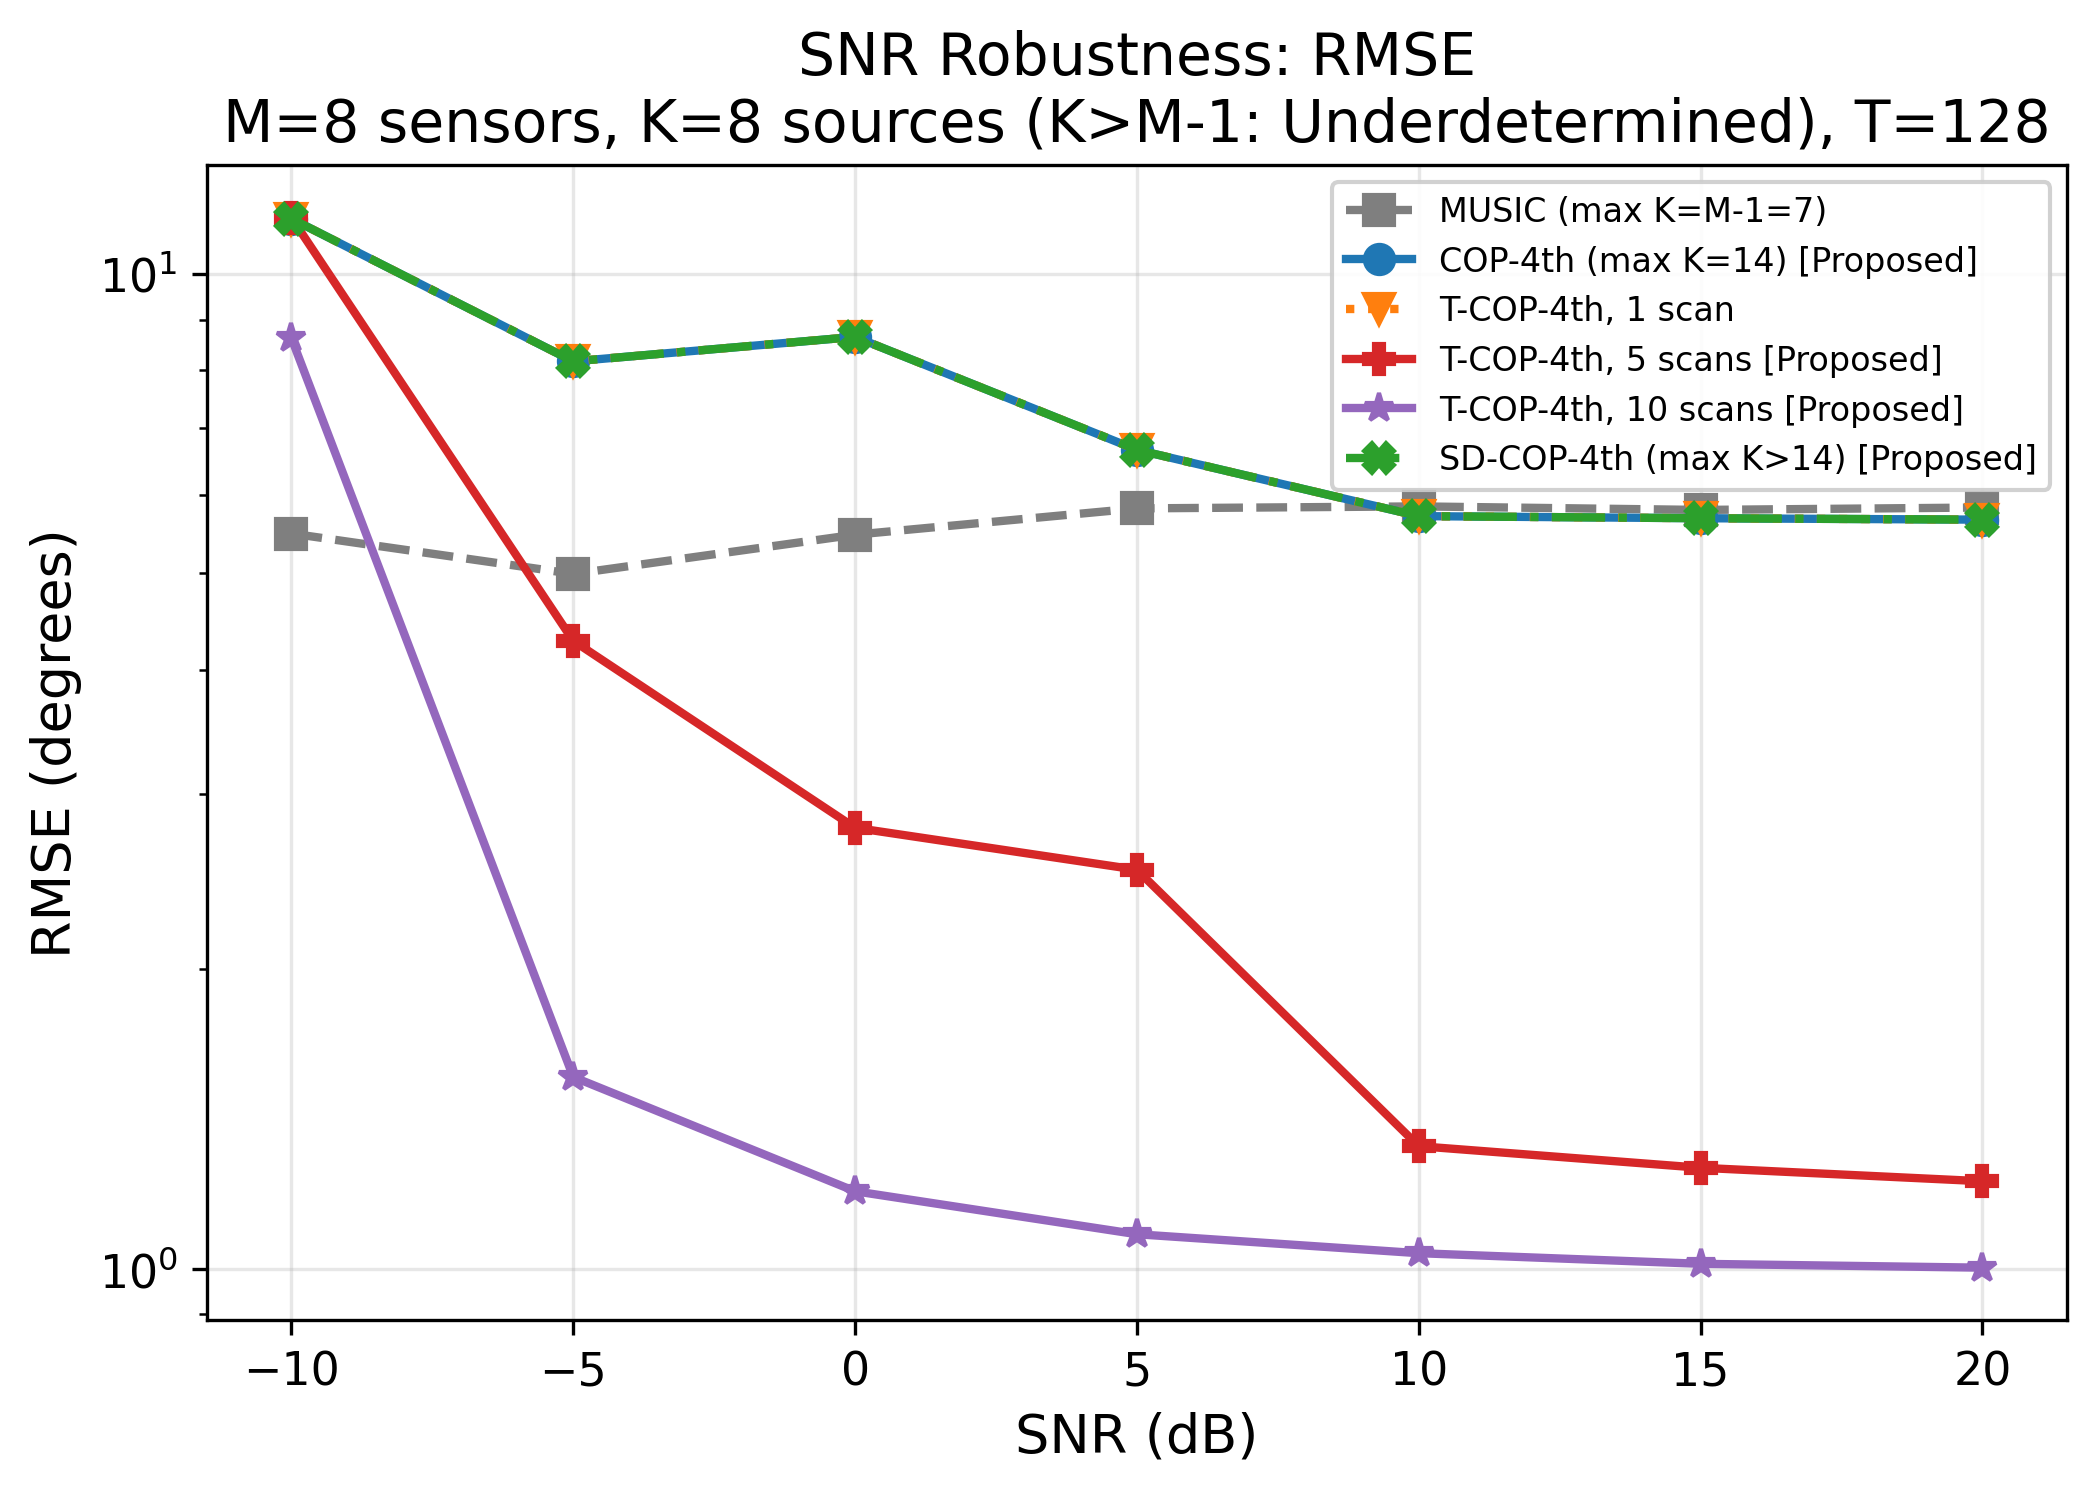
\includegraphics[width=\linewidth]{../results/figures/fig4_snr_rmse.png}
\caption{RMSE vs. SNR for $K = 8$ sources with $M = 8$ sensors (underdetermined). Dashed/dotted black lines show exact CRLB for standard and 4th-order estimation.}
\label{fig:snr}
\end{figure}

\subsection{Experiment 3: Angular Resolution}

\textbf{Setup}: $K = 3$ closely spaced sources at $\{-\Delta, 0, +\Delta\}$ degrees, spacing $\Delta \in [1^\circ, 15^\circ]$, SNR $= 15$~dB, $T = 512$.

Fig.~\ref{fig:resolution} demonstrates that COP-based methods achieve superior angular resolution compared to classical approaches. COP resolves sources down to $2^\circ$ separation, while MUSIC and Capon require $\geq 5^\circ$. T-COP with temporal accumulation further improves resolution to approximately $1^\circ$.

\begin{figure}[t]
\centering
\includegraphics[width=\linewidth]{../results/figures/fig5_resolution.png}
\caption{Close-spacing resolution: detection rate and RMSE vs. angular separation for $K = 3$ sources ($M = 8$, SNR $= 15$~dB).}
\label{fig:resolution}
\end{figure}

\subsection{Experiment 4: Snapshot Efficiency}

\textbf{Setup}: $K = 6$, SNR $= 10$~dB, $T \in \{32, 64, 128, 256, 512, 1024\}$.

Fig.~\ref{fig:snapshots} shows that COP requires approximately $T = 128$ snapshots to achieve stable estimation, while MUSIC requires $T \geq 256$ (and still fails due to the underdetermined configuration). T-COP achieves the best sample efficiency through temporal accumulation across scans. Both CRLB curves decrease with $\sqrt{T}$ as expected, with the 4th-order CRLB consistently below the standard CRLB.

\begin{figure}[t]
\centering
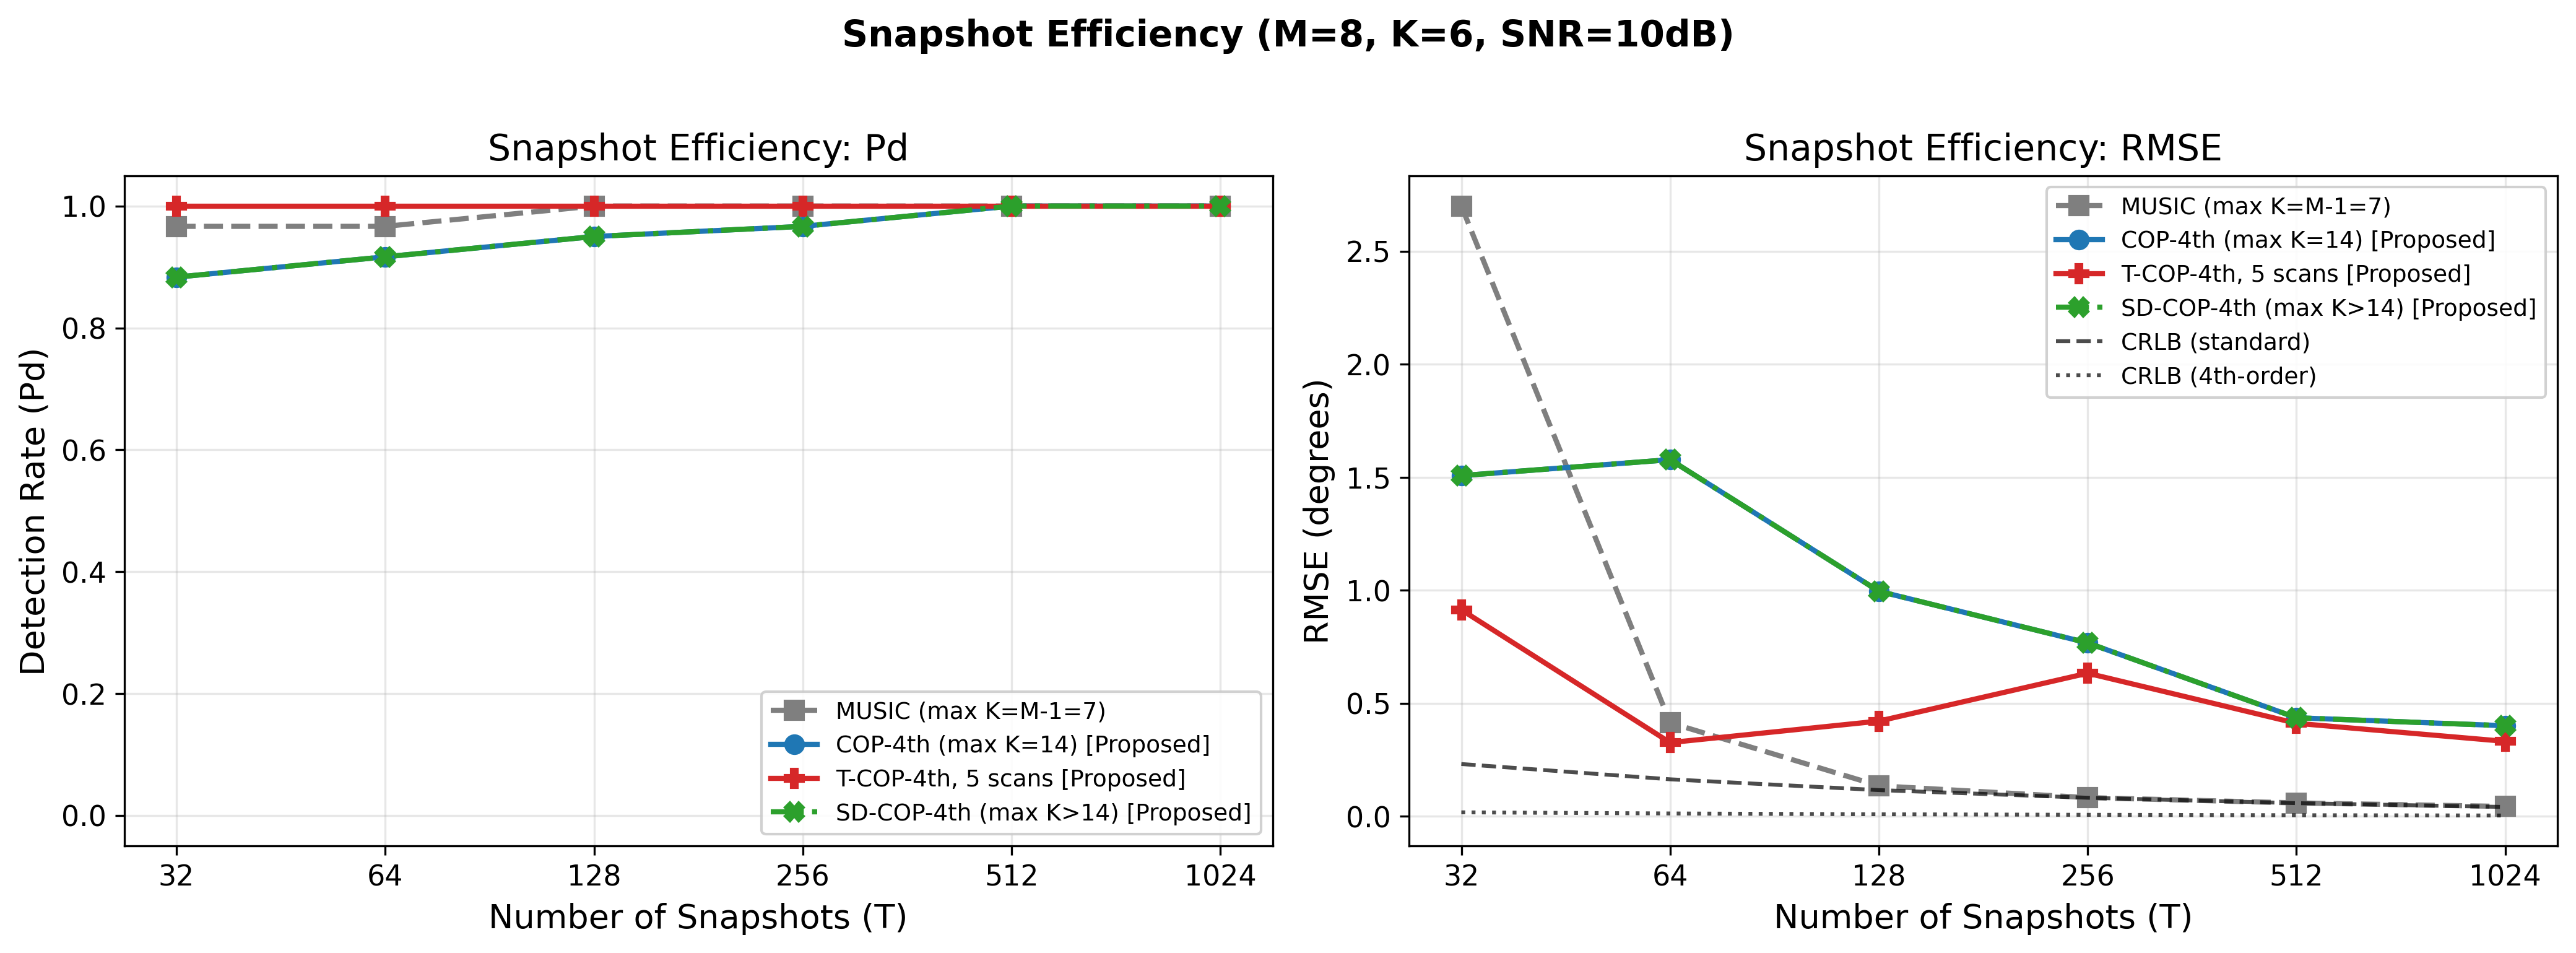
\includegraphics[width=\linewidth]{../results/figures/fig6_snapshots.png}
\caption{Snapshot efficiency: detection rate and RMSE vs. number of snapshots $T$ ($M = 8$, $K = 6$, SNR $= 10$~dB). CRLB curves shown as theoretical lower bounds.}
\label{fig:snapshots}
\end{figure}

\subsection{Experiment 5: SD-COP Extended Capacity}

\textbf{Setup}: $K = 10$ to $24$ sources, SNR $= 15$~dB, $T = 512$.

Fig.~\ref{fig:extended_k} focuses on the super-underdetermined regime. SD-COP maintains Pd $> 0.4$ up to $K = 24$ through multi-stage deflation, while single-stage COP drops to near-zero performance beyond $K = 14$. The number of deflation stages increases from 1 to 2--3 as $K$ exceeds the single-stage capacity.

\begin{figure}[t]
\centering
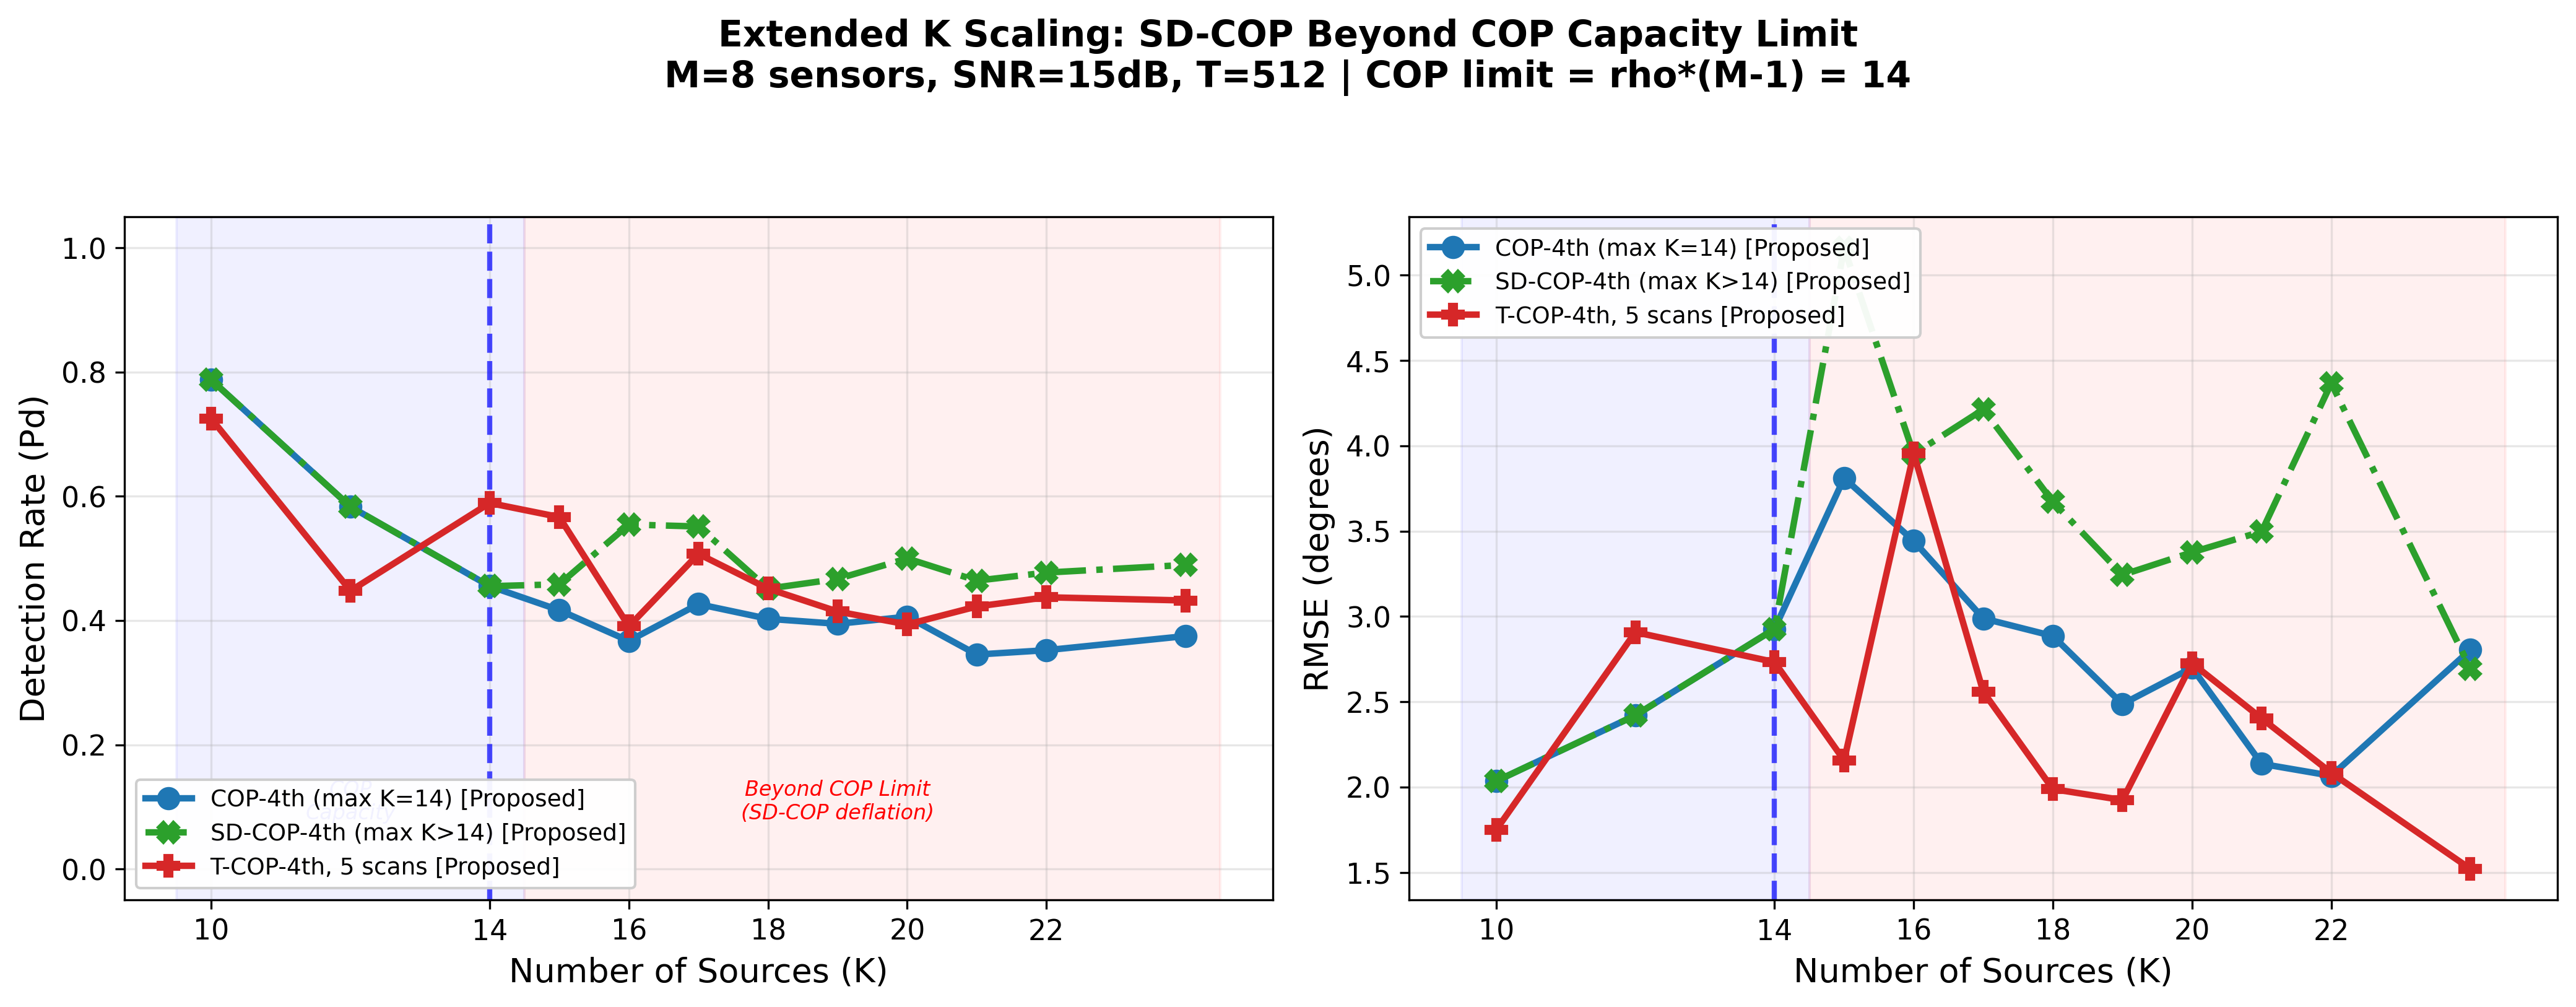
\includegraphics[width=\linewidth]{../results/figures/fig11_extended_k.png}
\caption{Extended K scaling: SD-COP performance beyond the single-stage COP limit ($K = 14$) through sequential deflation ($M = 8$, SNR $= 15$~dB).}
\label{fig:extended_k}
\end{figure}

\subsection{Experiment 6: Multi-Target Tracking with Birth/Death}

\textbf{Setup}: Time-varying target scenario where targets appear (birth) and disappear (death) over 20 scans. $M = 8$, SNR $= 15$~dB, $T = 256$. Target count varies from 1 to 5 and back.

Fig.~\ref{fig:birth_death} demonstrates the COP-PHD filter's ability to detect new targets within a single scan and maintain accurate cardinality estimation. The physics-based birth mechanism, which creates new tracks only from unassociated COP measurements, prevents false track initiation from clutter while enabling immediate detection of genuine new targets.

\begin{figure}[t]
\centering
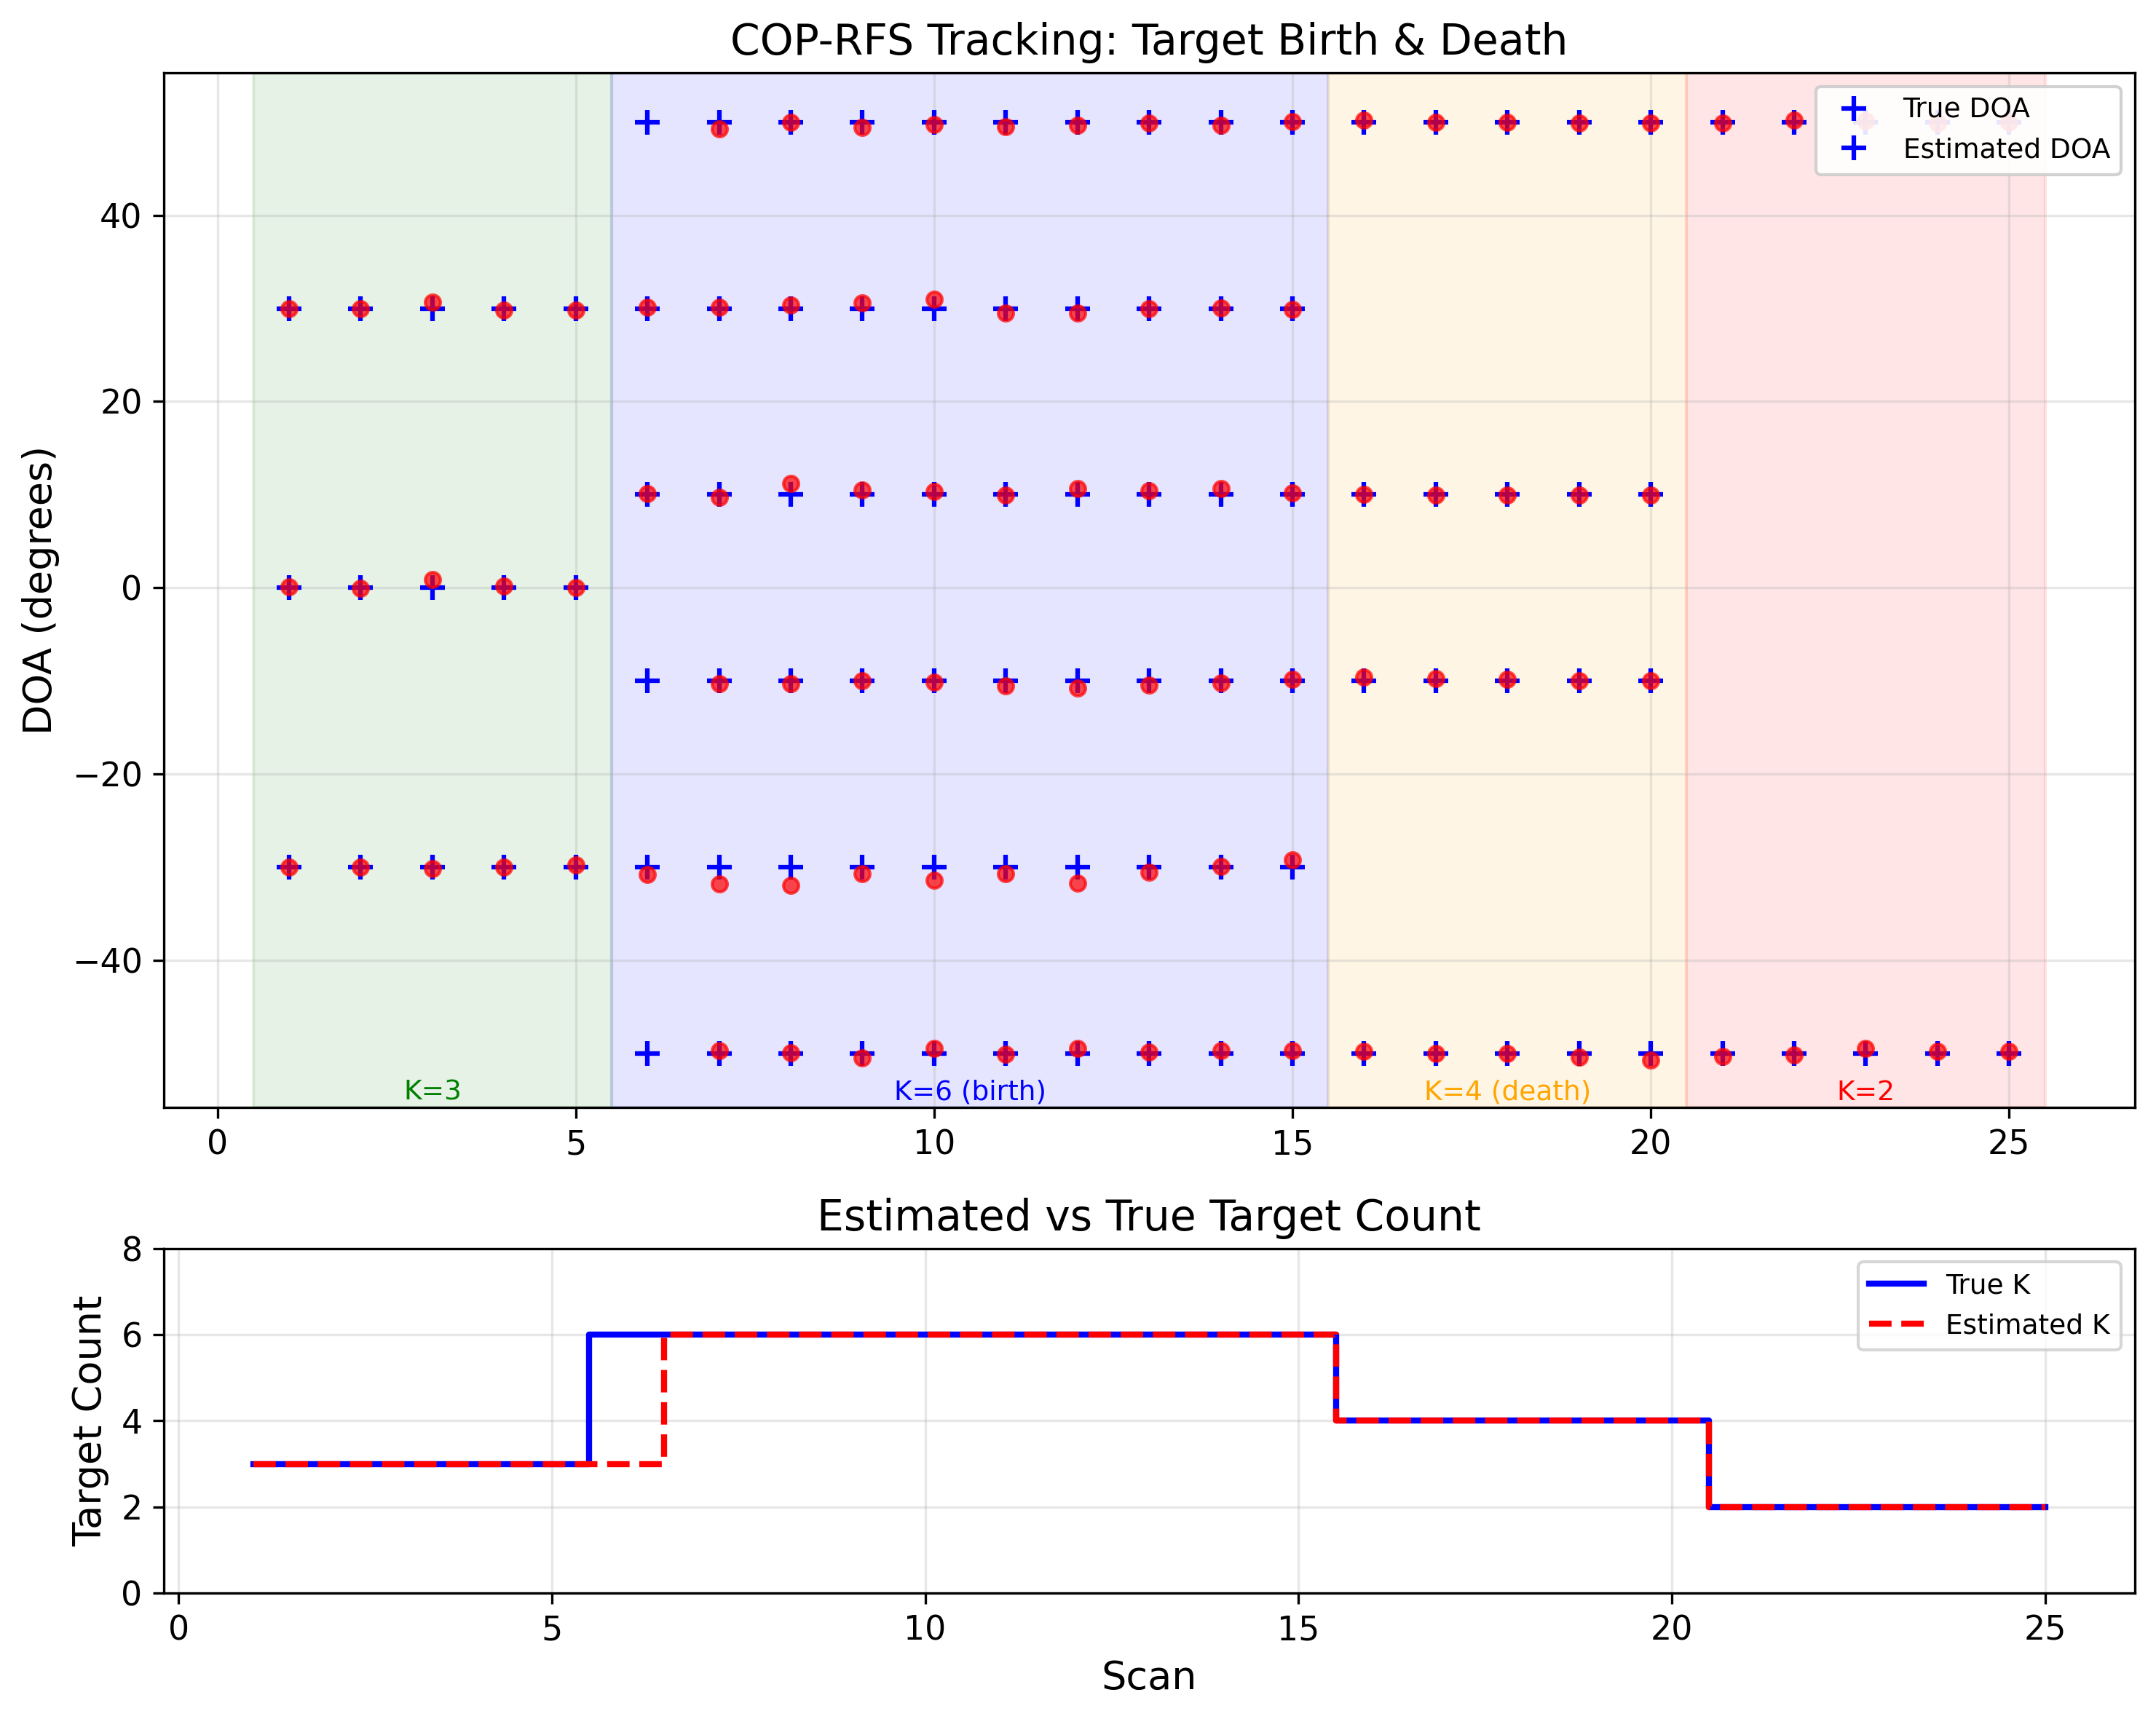
\includegraphics[width=\linewidth]{../results/figures/fig7_birth_death.png}
\caption{Multi-target tracking with time-varying target count: (a) DOA tracks, (b) cardinality estimation, (c) COP-PHD component evolution.}
\label{fig:birth_death}
\end{figure}

\subsection{Experiment 7: T-COP Feedback Loop}

\textbf{Setup}: 5 targets with the T-COP + PHD feedback loop. COP estimates feed the PHD tracker, which provides predicted DOAs back to T-COP for subspace refinement.

Fig.~\ref{fig:feedback} shows the RMSE convergence over scans. The tracker-aided T-COP (with feedback) converges faster and achieves lower steady-state RMSE than standalone COP, demonstrating the mutual benefit of the estimation--tracking feedback loop.

\begin{figure}[t]
\centering
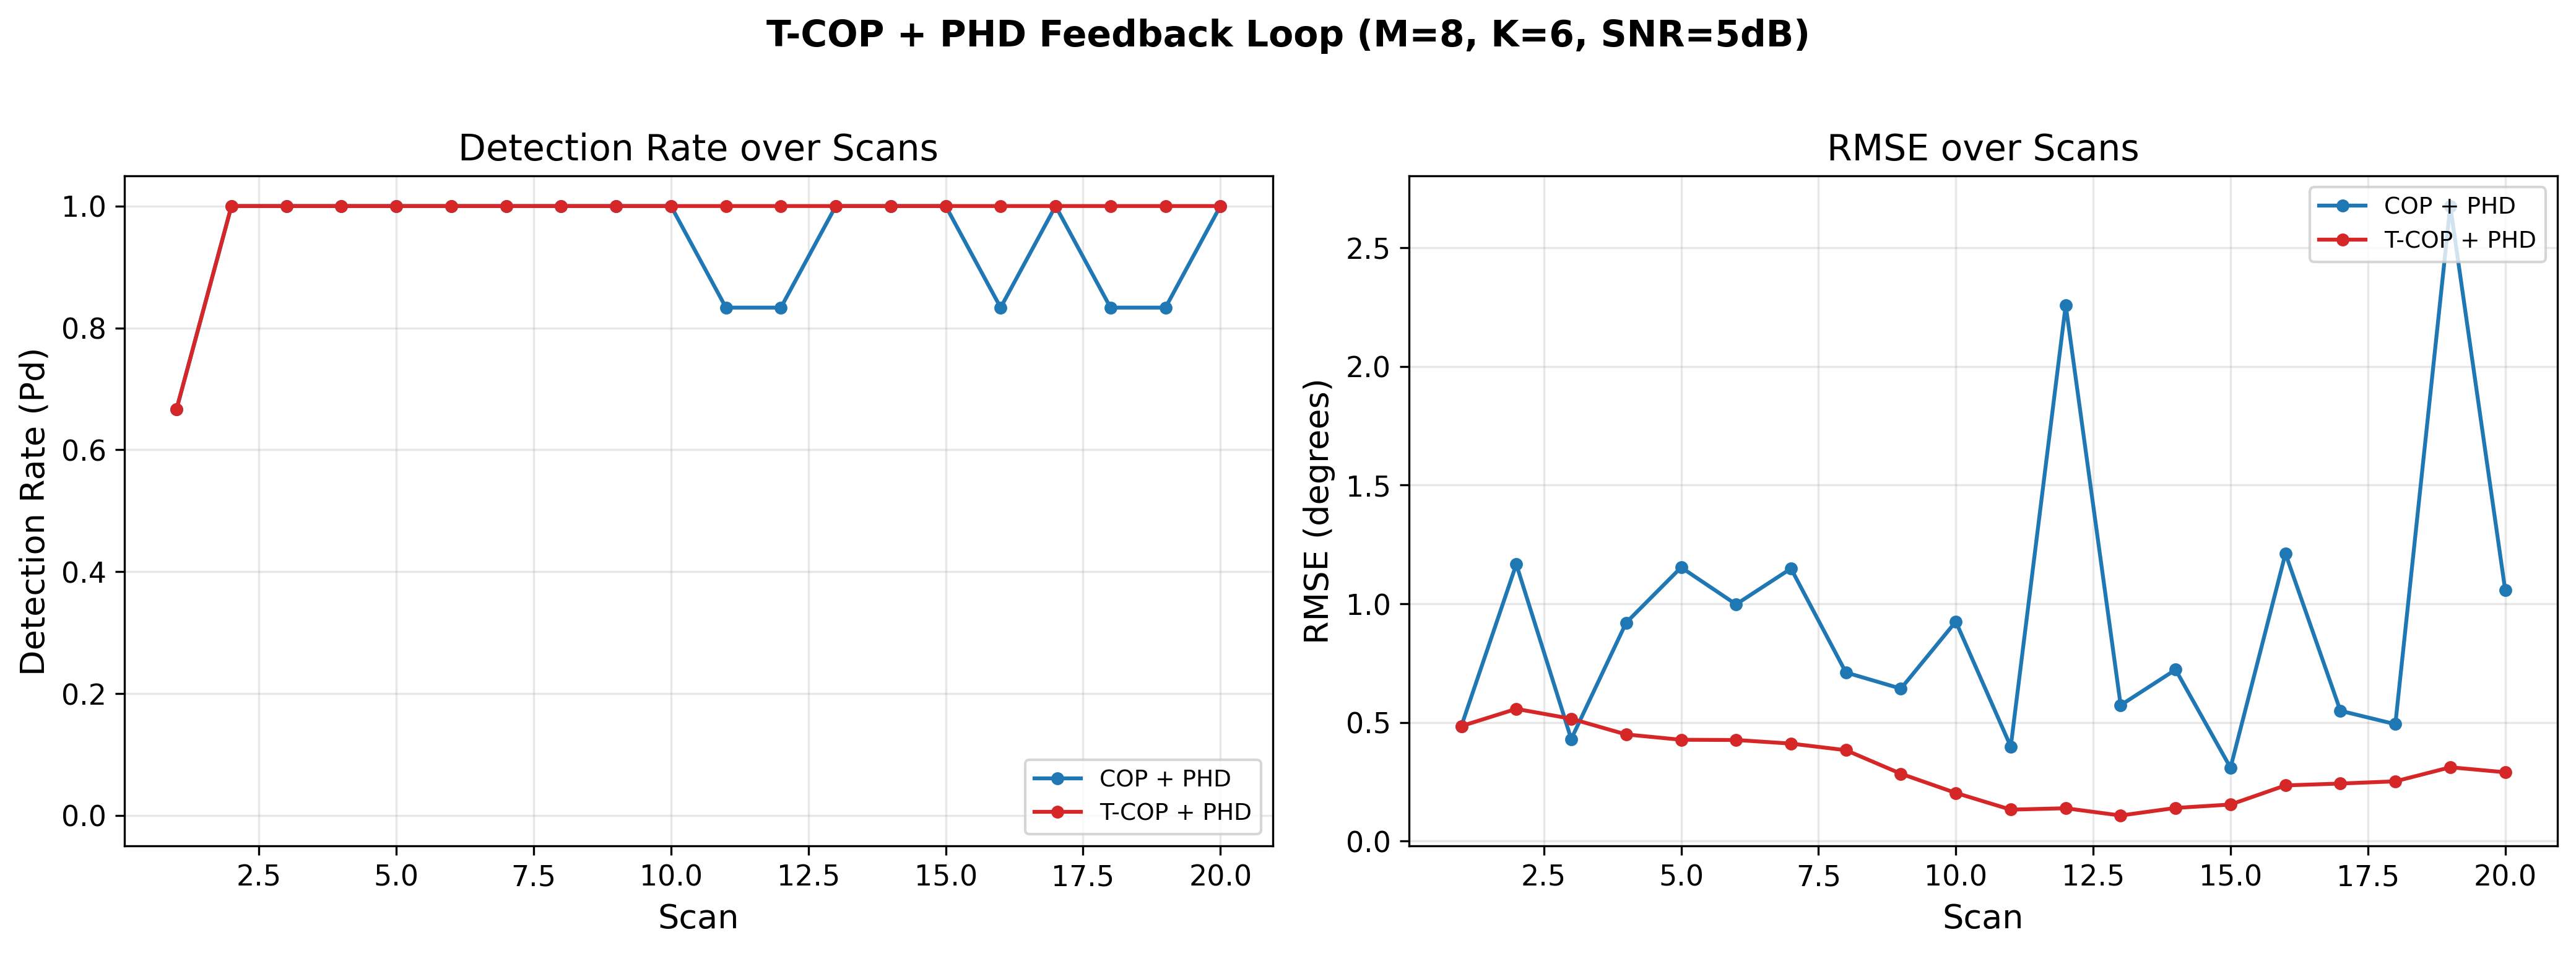
\includegraphics[width=\linewidth]{../results/figures/fig8_tcop_phd_feedback.png}
\caption{T-COP + PHD feedback loop: tracker-predicted DOAs refine cumulant subspace estimation, improving both estimation and tracking accuracy.}
\label{fig:feedback}
\end{figure}

\subsection{Experiment 8: Moving Target Tracking with Crossings}

\textbf{Setup}: 4 targets with constant-velocity trajectories that cross at scans $\sim$9 and $\sim$20, $M = 8$, SNR $= 15$~dB, $T = 512$, process noise $= 0.3^\circ$/scan.

Fig.~\ref{fig:moving_targets} presents the most challenging scenario. The physics-based GM-PHD filter achieves sub-degree RMSE ($< 0.5^\circ$) across all scans, \emph{including crossing points}. This is enabled by:
\begin{itemize}
\item \textbf{Velocity-gated merge}: Targets at the same position but with different velocities are not merged.
\item \textbf{Hungarian assignment}: Optimal measurement-to-prediction matching based on both position and velocity cost.
\item \textbf{Inertia-based prediction}: Targets continue on their predicted trajectories even when measurements are ambiguous at crossings.
\end{itemize}

\begin{figure}[t]
\centering
\includegraphics[width=\linewidth]{../results/figures/fig9_moving_targets.png}
\caption{Moving target tracking with trajectory crossings: physics-based identification maintains accurate track assignment through crossing points (scans $\sim$9 and $\sim$20).}
\label{fig:moving_targets}
\end{figure}


\subsection{Computational Complexity}

Table~\ref{tab:complexity} summarizes the computational complexity of the proposed algorithms compared to baselines.

\begin{table}[t]
\centering
\caption{Computational Complexity Comparison}
\label{tab:complexity}
\begin{tabular}{lcc}
\toprule
\textbf{Algorithm} & \textbf{Complexity} & \textbf{Limiting Factor} \\
\midrule
MUSIC & $\mathcal{O}(M^3 + NM^2)$ & EVD + spectrum \\
ESPRIT & $\mathcal{O}(M^3)$ & EVD \\
Capon & $\mathcal{O}(M^3 + NM^2)$ & Inversion + spectrum \\
COP-4th & $\mathcal{O}(M^4T + M_v^3 + NM_v^2)$ & Cumulant + EVD \\
T-COP & $\mathcal{O}(M^4T + M_v^3)$ & Cumulant + EVD \\
SD-COP & $\mathcal{O}(S \cdot (M^4T + M_v^3))$ & $S$ stages \\
GM-PHD & $\mathcal{O}(JM_n)$ & Components $\times$ meas. \\
\bottomrule
\end{tabular}
\end{table}

The cumulant computation $\mathcal{O}(M^4 T)$ dominates for COP methods, where the exponent $4$ corresponds to the fourth-order cumulant ($\rho = 2$). However, this overhead is justified by the $\rho$-fold increase in resolvable sources.


% ============================================================
\section{Conclusion}
\label{sec:conclusion}
% ============================================================

This paper presented COP-RFS, a unified framework for underdetermined high-resolution DOA estimation and multi-target tracking. Three novel extensions of the COP algorithm were proposed: T-COP for temporal accumulation with tracker feedback, SD-COP for capacity extension through sequential deflation, and a physics-based GM-PHD filter for robust tracking through target crossings.

The key contributions and findings are:
\begin{enumerate}
\item The COP family resolves $K > M-1$ sources using only $M$ sensors, with COP supporting up to $\rho(M-1) = 14$ sources and SD-COP extending this to $K > 20$ for $M = 8$.
\item T-COP's tracker-aided temporal accumulation creates a mutually beneficial feedback loop that improves both estimation and tracking accuracy, approaching the 4th-order CRLB with sufficient temporal averaging.
\item The physics-based predict--identify--update pipeline in the GM-PHD filter achieves sub-degree tracking RMSE through target crossings, where conventional approaches fail due to measurement--track ambiguity.
\item Exact CRLB derivations for both standard and higher-order cumulant-based DOA estimation confirm the theoretical advantage of the extended virtual aperture.
\end{enumerate}

The proposed framework is particularly relevant to defense applications where multiple incoming threats must be simultaneously detected, localized, and tracked using compact sensor arrays with limited aperture. Future work includes extension to two-dimensional (azimuth--elevation) DOA estimation, non-uniform array geometries, and real-time implementation on embedded radar platforms.


% ============================================================
% References
% ============================================================
\bibliographystyle{IEEEtran}
\bibliography{references}

\end{document}
